% 
%  $Author: awl8049 $
%  $Date: 2012/03/01 07:31:39 $
%  $Revision: 1.14 $
%
\documentclass[times, 10pt,twocolumn]{IEEEtran} 
\usepackage{amsmath,amsthm,amsfonts,amscd} % Some packages to write mathematics.
\usepackage{setspace}
\usepackage{pdfpages}
\usepackage{comment}
\usepackage{graphicx}
\DeclareGraphicsExtensions{.png,.jpg,.pdf,.eps}
\usepackage[caption=false,labelfont=sf,textfont=sf,captionskip=5pt]{subfig}
\graphicspath{{graphics/}}
\usepackage{authblk}
\usepackage{verbatim} % Allows quoting source with commands.
\usepackage{listings}
\usepackage{afterpage}
\usepackage[section]{placeins}
\lstloadlanguages{Matlab,C++,C,Pascal}
\lstset{
         basicstyle=\footnotesize\ttfamily, 
         %numbers=left,              
         numberstyle=\tiny,          
         %stepnumber=2,              
         numbersep=5pt,              
         tabsize=2,                  
         extendedchars=true,         
         breaklines=true,            
         keywordstyle=textbf,    
         stringstyle=\ttfamily, 
         showspaces=false,       
         showtabs=false,         
         xleftmargin=17pt,
         framexleftmargin=17pt,
         framexrightmargin=5pt,
         framexbottommargin=4pt,
         %backgroundcolor=\color{lightgray},
         showstringspaces=false  
 }
\usepackage{caption}
% \DeclareCaptionFont{white}{\color{white}}
% \DeclareCaptionFormat{listing}{\colorbox[cmyk]{0.43, 0.35, 0.35,0.01}{\parbox{\textwidth}{\hspace{15pt}#1#2#3}}}
% \captionsetup[lstlisting]{format=listing,labelfont=white,textfont=white, singlelinecheck=false, margin=0pt, font={bf,footnotesize}}
\newcommand{\equationname}{Eq.\ }
\newcommand{\equationnames}{Eq.\ }
\newcommand{\figurenames}{Figs.}
\setcounter{topnumber}{4}
\setcounter{bottomnumber}{2}
\setcounter{totalnumber}{5}
\renewcommand{\topfraction}{0.85}
\renewcommand{\bottomfraction}{0.85}
\renewcommand{\textfraction}{0.15}
\renewcommand{\floatpagefraction}{0.7}
\begin{document}
\title{Thermal-Aware Scheduling and Load Balancing Using Predictive
  Energy Consumption Models in High-Performance Multicore Systems} 
\author[]{Adam  Lewis} 
\author[]{Nian-Feng Tzeng} 
\affil[]{Center for Advanced Computer Studies, University of Louisiana at
  Lafayette, Louisiana 70504\\
  \{awlewis,tzeng\}@cacs.louisiana.edu }
\maketitle
\newtheorem{defn}{Definition}
\newtheorem{thm}{Theorem}
\thispagestyle{empty}
\begin{abstract}
  Modern processors crudely manage thermal emergencies through Dynamic
  Thermal Management (DTM), where the processor monitors the die
  temperature and dynamically adjusts the processor voltage and
  frequency (DVFS) to throttle down the processor when necessary. However, DVFS tends to
  yield marked degradation in both application performance and system
  reliability. Thus, pro-active scheduling techniques that avoid thermal
  emergencies are preferable over reactive hardware techniques like
  DTM.  Based on our previously introduced thermal Chaotic Attractor Predictors
  (CAPs, which take into account key thermal indicators and system
  performance metrics for overall energy consumption estimation within a
  given power and thermal envelope), we have developed and evaluated an
  effective thread scheduler for multicore systems.  Besides CAPs, our
  scheduler makes use of two basic principles to minimize server energy
  consumption: (1) selecting the thread with the least
  probability of causing a DTM in the subsequent time quantum,
  for executopm on the next available core, and (2) migrating
  execution threads on thermally overextended cores to
  other cool cores via load balancing so as to observe the thermal envelope.
  Our developed scheduler is evaluated in practice to
  assess its potential advantage resulting from thermal-awareness by
  incorporating CAPs (for temperature prediction) and basic principles
  (for energy reduction) into the existing scheduler in the FreeBSD
  operating system.   Our implemented scheduler is run on a server with
  the Intel Xeon processor for gathering measures of interest (including
  die temperature readings and execution times) when benchmark codes
  from the SPEC CPU2006 and PARSEC suites are executed.  The gathered
  results reveal that our proposed scheduling exhibits reduction
  in average core die temperatures by 3$^{\circ}$C\ to 6$^{\circ}$C\ under
  streaming benchmarks and by 10$^{\circ}$C\ to 12$^{\circ}$C\
  under other benchmarks, while causing only 1\% to 4\% performance degradation.
\end{abstract}

\section{Introduction}
\label{sec:Introduction}
Modern processors crudely manage thermal emergencies through Dynamic
Thermal Management (DTM), where the processor monitors the die
temperature and dynamically adjusts the processor voltage and frequency
(known as Dynamic Voltage and Frequency Scaling (DVFS))
to throttle down the processor whenever necessary. However, the use of
DVFS tends to cause significant negative impacts on application performance
and system reliability \cite{Donald2006,Bircher2008,Coskun2008d}.

This paper introduces effective scheduling for preventive thermal
management that minimizes server energy consumption by (1) 
selecting the subsequent thread with the smallest thermal impact
in the next time quantum to execute on an available core, and (2)
relocating threads run on thermally overextended cores
to other available cores for load balancing.
As opposed to prior pursuit of thermal-aware
scheduling \cite{Gomaa2004,Choi2007,Yang2008,Sarood2011} that 
aimed to bound temperatures below critical thresholds, our work considers
how to schedule high workload for die temperature management across all cores.

The current generation of operating systems treats those cores in 
multicore and virtualized multi-threaded processors (like those with Intel's HyperThreading technology) as distinct logical 
processors which are scheduled independently.
However, dependency and contention exist in shared resources 
among those logical processors, and hence they need to be taken into account upon their scheduling to address performance
and energy efficiency.
One approach based on software optimization at the application 
level aimed to make codes themselves more aware of existing
dependencies~\cite{Khan2011}.
While effective, such an approach may not be applicable in all 
cases and does not possess economies of scale.
It thus calls for the need of intelligent, thermal-aware load 
balancing and scheduling within the operating system,
achievable via modeling full-system energy consumption based on 
computational load for effectively predicting future energy 
consumption and its associated thermal change. 

To this end, we arrive at a thermal model which relates server energy consumption to the overall thermal envelope,
establishing an energy relationship between workload and
overall system thermodynamics.
According to our analysis of experimental measurements of
key processor performance counter readings and performance 
metrics, it is found that the measured readings and metrics
do not possess linearity and are \textit{chaotic in nature}.
Hence, our thermal model, based on a thermal Chaotic Attractor Predictor (tCAP),
takes into account key thermal indicators
(like ambient temperatures and die temperatures)
and system performance metrics (like performance counters)
for system energy consumption estimation within a given power and
thermal envelope.
This work demonstrates that effective scheduling can
result from taking advantage of our devised tCAP
when dispatching jobs to confine server power consumption
within a given power budget and thermal envelope while
avoiding detrimental impact upon server performance.

Dealing with all cores in a multicore system, 
a thermal-aware thread scheduler is highly dessirable to ensure that all of the cores in such a system
are kept equally busy, realized by migrating
threads over all the cores (no matter whether in the same processors or different ones)
when necessary for load balancing in the system.
Existing schedulers aid in processor thermal management by 
dispatching workloads to cores as tightly as possible
within the same proces$H$ sors to expose more opportunities
for power management via shutting down unused cores.  However,
computation-bound server workload fully utilizes available system
cores in most times, thereby rendering such schedulers ineffectual.
Our Thermal-Aware Scheduler (TAS) addresses this problem by 
thermally balancing system workload with as little performance degradation as possible.
TAS is demonstrated and evaluated by adding
thermal-awareness to the existing scheduler in the FreeBSD 
operating system executed on Intel Xeon (Woodcrest) processors.  
Subsets of SPEC CPU2006 and PARSEC benchmark suites which 
represent typical application server workloads,
are chosen to evaluate our TAS.

After an overview on pertinent background and related work is provided
in Section~\ref{sec:related}, this article introduces our proposed
thermal model in Section \ref{sec:model} and explains in Section
\ref{sec:therm-chaot-attr} how the model can be used for predictive
purposes.  Section~\ref{sec:sdesign} details the design of our TAS,
which is experimentally evaluated in Section~\ref{sec:experiment}, with
obtained evaluation results included and discussed as well.
Section~\ref{sec:conclusion} offers our conclusion.


\section{Background and Related Work}
\label{sec:related}
The kernel thread scheduler is responsible for placing threads in the
dispatch queue, deciding which thread to run on a processor
and managing the movement of threads to and from processors
so as to balance the workload amongst all cores.
A scheduler must fulfill this role while addressing two major applications requirements:
(1) making equal progress on all threads of a given application, 
and (2) exploiting as much hardware parallelism as
possible~\cite{Hofmeyr2010}. Traditional server load balancing
has varying assumptions about workload behavior when making thread placement decisions.  
In particular, interactive workloads are assumed to involve independent tasks that remain quiet for extended periods.  
Server workloads, on the other hand, are assumed to contain large numbers of threads
which are highly independent of each other and use synchronization objects to
ensure mutual exclusion on small data items. 
Modern operating systems (such as Linux and Solaris)
make load balancing more power-aware by placing 
workloads to cores as tightly as possible (inside fewest possible processors),
thereby presenting more opportunities for power management software to shutdown
unused resources \cite{Sun2009,Sun2009b,Xia2010}.

The following subsections describe in sequence,
background and prior work pertinent to thermal modeling,
scheduling with load balancing support, and chaotic behavior of energy comsumption
observed in our prior article.

\subsection{Thermal Modeling}
\label{sec:thermal-modeling}
All existing thermal models required to fit targeted mathematical expressions based on time-series observations of temperatures during the course of executing various workloads.
Expression coefficients were estimated by minimizing total least square errors between modeling results and actual temperature readings.
After proper calibration, such a mathematical expression becomes a model for extrapolating future temperatures.
Different modeling techniques have been devised.
In particular, a model based on integer linear programming was adopted by an earlier task scheduler [21], which aimed to meet real-time dealines while minimizing hot spots and spatial temperature differentials across the die.
Meanwhile, dynamic thermal modeling includes Heat-and-Run [4], HybDTM [19] and ThreshHot [6], [22].
Heat-and-Run distributes work among available cores until the DTM events arise, and it then migrates threads from the overheated cores to other cool cores.
On the other hand, HybDTM enhances DTM with a thread migration strategy which lowersthe priority of jobs executed on hot cores.
Separately, ThreashHot employs an on-line temperature estimator to determine the proper order to schedule threads across cores, favoring those threads which cause the greatest temperature hikes while avoiding DTM events to occur.
Schedulers based on prior thermal modeling all rely on readings of hardware performance counters and temperature sensors.
They can be improved by analyzing on-die thermal variations to aid in system power and thermal management [17], [23], [24].

However, preceding techniques all react to the temperature approaching the
DTM threshold rather than trying to avoid reaching that temperature in
the first place.  A proactive solution with multi-tier prediction was suggested in
Ayoub~\textit{et al.}\ \cite{Ayoub2011}, where a
core level predictor was employed to convert temperature observations to operating frequency estimates
while a control-theoretic based scheduler was followed at the socket level for process level scheduling.
Separately, a scheduling policy for sorting the tasks in each core's run queue according to
memory intensity was considered  so as to schedule memory-bound tasks at slower frequencies
\textit{et al.}\ \cite{Merkel2008b,Merkel2010}.  
Later, the process scheduling policy was modified in \cite{Bellosa2003} to allocate time slices
following (1) the contribution of each task to the system power consumption and
(2) the current processor temperature.  
A similar approach made use of idle cycle injection to manage CPU time slice allocation,
aiming to maintain a lower average temperature over time,
as opposed to managing temperatures against a critical threshold.
Meanwhile, Cool Loop \cite{Choi2007} and Dimentrodon \cite{Bailis2011} address a lack of heat slack
by inserting additional cycles into the task scheduling to create
thermal slack, naturally leading to performance degradation.
A variation of preceding schemes relied on system level compiler support to
insert a run-time profiling code into applications 
for providing hints on the thermal intensity of a task \cite{LiK2008}.  
However, such an approach works ineffectively under many server
cases where the available slack in deadlines does not exist.

\subsection{Earlier Scheduling with Load Balancing Support}
\label{sec:therm-comp-workl}
Modern multiprocessor operating systems (such as Windows, Linux, Solaris,
and FreeBSD) often take a two-level approach to task scheduling for
maximized system resource utilization.
Such an approach uses a distributed run queue model for managing each core
at the first level, with per core queues and fair scheduling policies.
Its second level balances the work load by redistributing tasks across the queues.  
In particular, the FreeBSD ULE scheduler
\cite{Roberson2003,McKusick2004,McKusick2004b} uses a combination of
push and pull thread migration for load balancing. 
\textit{Push migration} scans the run queues associated with each processor
every 500 milliseconds to pick the most-loaded and least-loaded logical
processors before equalizing their run-queues. 
The processor then attempts to pick a core in the
same processor group so as to minimize the migration cost.
In \textit{pull migration}, a processor checks if its ahs excess work in
its run queue and also if another processor in the system is idle,
before adding new tread to its run queue.
The existence of an idle processor triggers an inter-processor interrrupt
to migrate the new tread to the idel processor.
Such two-level schedulers work under three assumptions:
(1) threads are independent, (2) load is governed by queue length,
and (3) locality exists and is important \cite{Hofmeyr2010}.
In practice, however, common servers often characterized as follows:
(1) their threads are logically related, with data and control dependencies among threads, 
and (2) their threads have equally long life spans \cite{Hofmeyr2010},
rendering previous two-level scheduling ineffective.

Meanwhile, existing operating systems have made their load balancing schemes
more power-aware by taking advantages of their power management drivers
which intend to find as compact an allocation
of processes to run-queues as possible \cite{Sun2009,Sun2009b,Xia2010,Sarood2011}.
This way presents more opportunities for the power management
software to shutdown unused resources. 
Such power-aware load balancing, while effective for interactive workloads,
works only if system resources are not completely utilized;
it becomes unviable if the system workload is high (common to high-performance servers).

\subsection{Chaotic Behavior of Energy Comsumption}
\label{sec:chaot-pred-energy}
An analytical model of server energy consumption was built earlier
\cite{Lewis2008,Lewis2010} by modeling energy consumption as a
function of the work done by the system in executing its computational
tasks and of residual thermal energy given off by the system in doing
that work.  The resulting dynamic system expresses energy consumption in
the time domain as follows:
\begin{equation}
  \label{eq:system}
  E_{system}=f(E_{proc},E_{mem},E_{em},E_{board},E_{hdd})
\end{equation}
where each of the terms in the above equation is defined as: (1)
$E_{proc}$: energy consumed in the processor due to computations, (2)
$E_{mem}$: energy consumed in the DDR SDRAM chips, (3) $E_{em}$: energy taken by the
electromechanical components in the system, (4) $E_{board}$:
energy consumed by peripherals that support the operation of the board,
and (5) $E_{hdd}$: energy consumed by the hard disk drive during the
system's operation.

The continuous system in \equationnames~\eqref{eq:system} can be viewed as a
multi-variate differential equation in the time domain that can be
estimated using a time series representation. This time series is
constructed by considering (1) an initial energy state $E_{system}$ at
time $t=0$ and (2) a set of physical predictors that approximate the
values of $E_{proc}$, $E_{mem}$, $E_{board}$, and $E_{hdd}$ at the next
interval $t+\Delta t$.  The result is a time series
\begin{equation}
\label{eq:tseries}
\hat{E}_{sys}(t)=\hat{f}(e\_proc_{t},e\_mem_{t},e\_em_{t},e\_board_{t},e\_hdd_{t})
\end{equation}
where each of quantities $e$ corresponds to one or more physically
observable predictors of the quantities in Eq.~\eqref{eq:system}. The
function $\hat{f}$ captures the method used to combine the physical
observations into $\hat{E}_sys$.  We place two requirements upon
$\hat{f}$: (1) it must quickly compute estimates to be suitable for
real-time prediction of energy and temperature changes, and (2) it must
approximate the behavior of the original function $f$ to an acceptable
accuracy.
\begin{figure}[tbph]
  \centering
  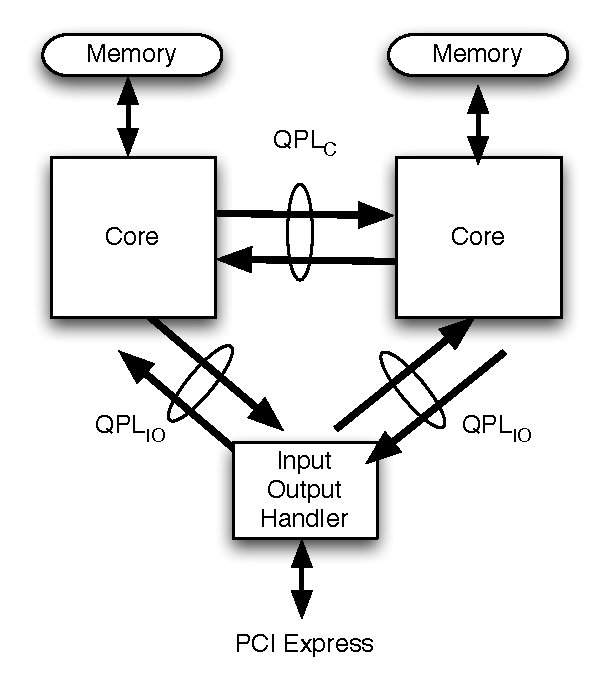
\includegraphics[scale=0.5]{intelnehalem}
  \caption{Intel Xeon (Woodcrest) architecture.}
  \label{fig:intarch}
\end{figure}
\begin{table}[tbhp]
  \centering
  \caption{PeCs and performance metrics for Intel Xeon server}
  \label{tab:intelmodel}
  \begin{tabular}{r l}
\hline
\textbf{Variable}&\textbf{Measurement}\\
\hline
$T_{C_{0}}$&Core 0 Die Temp\\
$T_{C_{1}}$&Core 1 Die Temp\\
$T_{C_{2}}$&Core 2 Die Temp\\
$T_{C_{3}}$&Core 3 Die Temp\\
$QPL_{C}$&Transactions on the QPLs between Cores\\
$QPL_{IO}$&Transactions on QPLs for IO Handler\\
$CM_{0}$&Last-level Cache Misses due to Core 0\\
$CM_{1}$&Last-level Cache Misses due to Core 1\\
$CM_{2}$&Last-level Cache Misses due to Core 2\\
$CM_{3}$&Last-level Cache Misses due to Core 3\\
$D_{r}$&Disk bytes read\\
$D_{w}$&Disk bytes written\\
$T_{A_{0}}$&Ambient Temp 0\\
$T_{A_{1}}$&Ambient Temp 1\\
$T_{A_{2}}$&Ambient Temp 2\\
$F_{C}$&Memory Cooling Fan Speed\\
$F_{M2a}$&Memory Cooling Fan Speed 2a\\
$F_{M2b}$&Memory Cooling Fan Speed 2a\\
$F_{M3a}$&Memory Cooling Fan Speed 3a\\
$F_{M3b}$&Memory Cooling Fan Speed 3b\\
$F_{M4a}$&Memory Cooling Fan Speed 4a\\
$F_{M4b}$&Memory Cooling Fan Speed 4b\\
$F_{M5a}$&Memory Cooling Fan Speed 5a\\
$F_{M5b}$&Memory Cooling Fan Speed 5b\\
$IR$&Instructions Retired \\
\hline
  \end{tabular}
\end{table}
Observations from each time series are measured using (1)~the appropriate
PeCs for the targeted processor (2)~operating system kernel virtual memory
statistics, and (3)~processor die temperatures and chassis ambient
temperatures.  Seventeen server measures are input to our
predictor, as listed in Table~\ref{tab:intelmodel}.  They are classified
into five groups, each associated with one server energy contributor.
Notice that $QPL_{C}$ and $QPL_{IO}$ are relevant to QuickPath Links
(depicted in \figurename~\ref{fig:intarch}), and they are associated
with $E_{proc}$ and $E_{mem}$, respectively.  In practice, however,
there is just one single PeC for holding aggregated $QPL_{C}$ and
$QPL_{IO}$ together.  Among those measures listed in
Table~\ref{tab:intelmodel}, the top three are pertinent to $E_{proc}$,
comprising $MP_{proc}$.  The next three measures determine $E_{mem}$,
forming $MP_{mem}$.  Those two $CM_{i}$ measures indicate the total L3
cache miss counts due to Core \textit{i}, $i$ = 0,1,2, or 3.  The cache
miss counts record the last-level cache (i.e., L3) misses for the Intel
Xeon processor on which our testing Intel server is built.  The next two
measures are related to $E_{hdd}$ (and constitute $MP_{hdd}$),
signifying the total numbers of bytes in disk reads and disk writes,
respectively, during a period of 5 seconds.  The subsequent three
measures dictate $E_{board}$, obtained from 3 temperature sensors placed
on the board for ambient temperature readings; they form $MP_{board}$.
Finally, the last nine measures determine $E_{em}$, offering speed
information of those nine memory cooling fans, to constitute $MP_{em}$.
As a result, each observation for the Intel server at time $t$ comprises
the 24 measures of $MP(t) =\left[MP_{proc}, MP_{mem}, MP_{hdd},
  MP_{board}, MP_{em}\right]^{T}$.  Application length is estimated in
each time period by the quantity $IR$, the total number of instructions
retired by the processor for this process.

A analysis on the data collected from our test systems indicates that
the temperature measurements and associated thermal metrics demonstrate
\textit{chaotic behavior}. A chaotic process is one which is highly
sensitive to a set of initial conditions.  Small differences in those
initial conditions yield widely diverging outcomes in such chaotic
systems.  In order to determine whether a process is chaotic, we must be
able to show that (1) it demonstrates high sensitivity to initial
conditions and topological mixing, and (2) its periodic orbits are dense
\cite{Sprott2003}.  

The time series approximation of a system solution for
\equationname~\eqref{eq:tseries} can be a viewed as a projection of the
flow of each equation onto a surface \cite{Liu2010}.  This projection is
defined so that the behavior of the dynamic system is reflected in our
discrete approximation.  The function $\hat{f}$ is expressed in terms of
a Chaotic Attractor Predictor (CAP), a linear least squares regression
of a multivariate local polynomial of degree $r$. A local constant
approximation for $\hat{f}$ is defined next in terms of a locally
weighted average \cite{Box1994} over the next $n$ observations, based on
the prior $p$ observations of $X_{t-1}, \ldots, X_{t-p}$ (each with $r$
metric readings):
\begin{equation}
\label{eq:fhatest}
    \hat{f}(x)=\dfrac{\displaystyle\sum_{t=p+1}^{n+p}O_{p}*K_{H}(X_{t-1}-x)}{\displaystyle\sum_{t=p+1}^{n+p}K_{H}(X_{t-1}-x)}
\end{equation}
with $O_{p}=(X_{t-1},\ldots,X_{t-p})^{T}$. 


\subsection{Limitations of Existing Scheduling}
\label{sec:shortc-comp-workl}
Current power management software that utilizes DVFS techniques to address DTM
events has been effective in addressing thermal emergencies
\cite{Donald2006,Hanson2007}, commonly implemented in modern server
processors \cite{AMD2007,Intel2009}.
However, handling DTM through DVFS can be problematic due to issues with
program phase behavior and contention for shared resources
\cite{Bircher2008,Coskun2008d}, resulting directly from
slow transitions between the active and the idle device states
and also from inability to access resources associated with idle processors.
When the power phase changes frequently, abundant thermal variations among cores
with the processor occurs, leading to decreased reliability \cite{Rosing2007,Coskun2008d,Kursun2009}.  For example, the Intel XScale processor was reported to decrease
its component MTTF (Mean Time to Failure) by 12\% to 34\%,
depending upon the selected power management strategy \cite{Rosing2007}. 

Work migration for energy savings and thermal management has a long
history in the SMP, SMT, and CMP environments \cite{Yao1995,Gomaa2004,Kumar2006,Yang2008}.
A study of OS-level thermal
migration using Linux on the IBM POWER5 processor~\cite{Choi2007}
discovered that the rise and fall times of core temperatures vary in the
order of hundreds of milliseconds.  
As most operating systems choose
scheduler ticks to be of 10 ms or less, it often is impossible to
react to thermal conditions before a critical state is reached.  
As a result, three improvement mechanisms for managing thermal states have been pursued:
(1) core hopping for leveraging spatial heat slack, (2) task scheduling
for leveraging temporal heat slack, and (3) SMT scheduling for
leveraging temporal heat slack.
In the presence of slack, each of those mechamisms may 
reduce core die temperatures by 3 to 5$^{\circ}$ C on an average,
at the expense of 3\% mean performance degradation ~\cite{Choi2007,Ayoub2009}.
However, in the absence of slack commonly found under heavy workloads in
high-performance servers, the three mechanisms becomes ineffective,
calling for suitable scheduling with thermal awareness proactively.

\section{System Thermal Model}
\label{sec:model}
In this section, we introduce a system thermal model built upon
what was reviewed in Section \ref{sec:chaot-pred-energy} to
address the thermal domain by first considering how to extend
\equationname~\eqref{eq:system} to account for the energy consumed by
executing an application.  
Two metrics are defined to account for the thermal impact of executing the
application.

The length $L(A,D_{A},t)$ of an application $A$ is the total execution time of
$t$ under the data set of $D_{A}$.
An application is composed of $p$ execution threads, each associated with
a data set sized $d_{i}$, for $1\leq i \leq p$,
in a processor. The total data associated with $A$ is the sum of
the data associated with its component thread:
\begin{equation}
\label{eq:totaldata} D_{A}=\displaystyle\sum_{i=1}^{p}{d_i}.
\end{equation} 
We assume that the activities take place in a staging
area which contains the main and virtual memory operating spaces, as
well as the processor with its cores and their associated caches and
shared cache.  This measurement of execution time includes both
computation time and the time to move application data from the
staging area (peripherals off the chip like DRAM and HDD) to a
computation or operation area (on the chip, such as the caches and the cores).

Each application $A$ with the problem size of $D_{A}$ involves
workload $W(p_{i},d_{i},t)$, for $1 \leq i \leq p$, consisting of two components: 
(1) a count of the operations performed by the computational core, 
and (2) the count of communication operations required for transfer of data,
instructions, and data coherency and book-keeping functionity. 
They are measured in terms of the number of bytes operated upon or transferred over.
Thus, energy consumed by executing application $A$
with data set $D_{A}$ can be expressed as:
\begin{equation}
\label{eq:eworkload} E_{A}(A,D_{A},t) = \displaystyle \lim_{n \to k_{e}
}n (p_{i},d_{i},t) L_n(A_{n},D_{A_{n}},t),
\end{equation}
for $1\leq i \leq p$, where $k_{e}$ is the total
number of applications that can be executed with the associated length
of time for $L_{n}$, at which point a ``thermal event'' will occur
to cause a catastrophically failure at the system and a system shutdown.

In order to relate system energy expenditure upon
application execution, to corresponding joule heating, we define the term
``Thermal Equivalent of Application'' (TEA), as the
electrical work converted to heat in running the application,
measured in terms of die temperature change and ambient temperature
change of the system. 
Hence, TEA of application $A$ is expressed by:
\begin{equation}
\label{eq:tea} \theta(A,D_{A}, T,t) =
\frac{E_{A}(A,D_{A},t)}{\displaystyle \lim_{T \to T_{th}} J_e (T -
T_{nominal})},
\end{equation} 
where $T_{th}$ denotes the threshold temperature
at which a thermal event will occur, whereas $T_{nominal}$ refers to the
nominal temperature as reported by the system when it is in a quiescent
state, i.e., only the operating system is running without any application execution.
The term $J_{e}$ is the ``electrical equivalent of
heat'' for the chip, which reflects the \textit{informational
entropy}\index{ientropy} of the system due to processing the
data bits during application execution and to the
black body thermal properties of the chip packaging as well as the cooling
mechanisms around the chip. Thus, TEA is a dimensionless quantity, with
both denominator and numerator expressing work done or energy consumed
in finishing an application.

We combine these metrics into achieved performance per unit power
consumed by the chip:
\begin{equation}
\label{eq:thermcost} C_{\theta}(A, D_{A}, T,t)=\frac{\Theta(A,D_{A}, T,
t)}{E_{sys}(A,D_{A},t)}
\end{equation} where $E_{sys}(A,D_{A},t)$ is the overall power consumed
during the application lifetime. This normalized quantity indicates the
``cost'' of executing an application on the given chip.  We can
apportion the total power consumed by a single physical component
(processor, DRAM units, HDD, motherboard, and
electrical/electromechanical) during the length $L_{A}$ of the
application by applying \equationname~\eqref{eq:system} to
\equationname~\eqref{eq:thermcost}.
\begin{table}[tbhp] \centering
  \caption{Intel Xeon PeCs used to estimate $\theta$ and $C_{\theta}$}
  \label{tab:tcappecs}
  \begin{tabular}{r l} \hline \textbf{Variable}&\textbf{Measurement}\\
\hline \textit{Application Length}&\\ $IR$&Instructions Retired \\
\textit{Data Set Size}&\\ $QPL_{C}$&Transactions on the QPLs between
Cores\\ $QPL_{IO}$&Transactions on QPLs for IO Handler\\
$CM_{0}$&Last-level Cache Misses due to Core 0\\ $CM_{1}$&Last-level
Cache Misses due to Core 1\\ $CM_{2}$&Last-level Cache Misses due to
Core 2\\ $CM_{3}$&Last-level Cache Misses due to Core 3\\ $D_{r}$&Disk
bytes read\\ $D_{w}$&Disk bytes written\\ \textit{System temperature}&\\
$T_{A_{0}}$&Ambient Temp 0\\ $T_{A_{1}}$&Ambient Temp 1\\
$T_{A_{2}}$&Ambient Temp 2\\ \hline
  \end{tabular}
\end{table}
\subsection{Thermal Chaotic Attractor Predictors}
\label{sec:therm-chaot-attr} Following the procedure reviewed in
Section~\ref{sec:chaot-pred-energy} (and detailed in \cite{Lewis2010}),
we map observable PeCs listed in Table~\ref{tab:intelmodel} to each of
the quantities in \equationname~\eqref{eq:tea} and
\equationname~\eqref{eq:thermcost} (as shown in
Table~\ref{tab:tcappecs}). The result is a pair of thermal Chaotic
Attractor Predictors (tCAPs) that can be used to predict the thermal
behavior of the application.

We performed an analysis on the data collected from our test systems to
confirm that the behavior of the time series representations can be
attributed to some form of chaotic behavior.  In order to evaluate a
server's sensitivity to initial conditions, we consider the Lyapunov
exponents of the time series data observed while running those
benchmarks described in the previous section.  The Lyapunov exponent
quantifies the sensitivity of a system such that a positive Lyapunov
exponent indicates that the system is chaotic \cite{Sprott2003}.  The
average Lyapunov exponent can be calculated using $\lambda =
\lim_{N\to\infty}\frac{1}{N}\sum_{n=0}^{N-1}ln|f'(X_n)|$.  We found a
positive Lyapunov exponent when performing this calculation on our data
set, ranging from 0.019 to 0.051 on our Intel test server, as listed in
Table~\ref{tab:chaotic}. Therefore, our data has met the first and the
most significant criterion to qualify as a chaotic process.

The second indication of the chaotic behavior for the time series
approximations expressed by Eqs.~\eqref{eq:tea} and
\eqref{eq:thermcost} is an estimate of the Hurst parameter $H$ for the
time series observations. If the value of the Hurst
parameter is greater than $0.5$, an increment in the random process is
positively correlated and long range dependence exists in the case of
time series \cite{Sprott2003}.  In a chaotic system, a value of $H$ approaching 1.0
indicates the presence of self-similarity in the system.  As
demonstrated in Table~~\ref{tab:chaotic}, the time series data collected
in our experiments all have $H$ values close to 1.0, ranging from
0.95 to 0.99 for the Intel server in our test environment.
\begin{table}[tbhp]
  \caption{Chaotic behavior in core die temperature time series}
  \label{tab:chaotic} 
   \centering 
% BEGIN RECEIVE ORGTBL chaosmeasures
\begin{tabular}{lrr}
\hline
 & Hurst Exp. ($H) & Lyaponov Exp. ($\lambda$) \\
 \hline
Core 0 & 0.99 & 0.051 \\
Core 1 & 0.98 & 0.019 \\
Core 2 & 0.97 & 0.034 \\
Core 3 & 0.95 & 0.040 \\
\hline
\end{tabular}
% END RECEIVE ORGTBL chaosmeasures
\begin{comment} 
#+ORGTBL: SEND chaosmeasures orgtbl-to-latex :splice nil :skip 0 
|--------+------------------+----------------------|
|        | Hurst Exp. ($H$) |    Lyaponov Exp. ($\lambda$) |
|--------+------------------+----------------------|
| Core 0 |            0.99  |               0.051  |
| Core 1 |            0.98  |               0.019  |
| Core 2 |            0.97  |               0.034  |
| Core 3 |            0.95  |               0.040  |
|--------+------------------+----------------------|
\end{comment}
\end{table}

\section{A Thermal Aware Scheduler}
\label{sec:sdesign} The scheduler in an operating system is responsible
for making two decisions in each time quantum: (1) thread scheduling,
i.e., deciding the next thread to run on a processor and (2) load
balancing, namely, distributing workload evenly across all cores, with
existing implementations mostly focusing on performance.  Our Thermal Aware
Scheduler incorporates a heuristic scheduling algorithm in a popular scheduler
(i.e., ULE in the FreeBSD operating system) for thermal stree reduction
on a multicore processor while meeting the SPMD requirements of
equal execution progress and maximum parallelism exploitation.

\begin{figure}[btph] \centering
  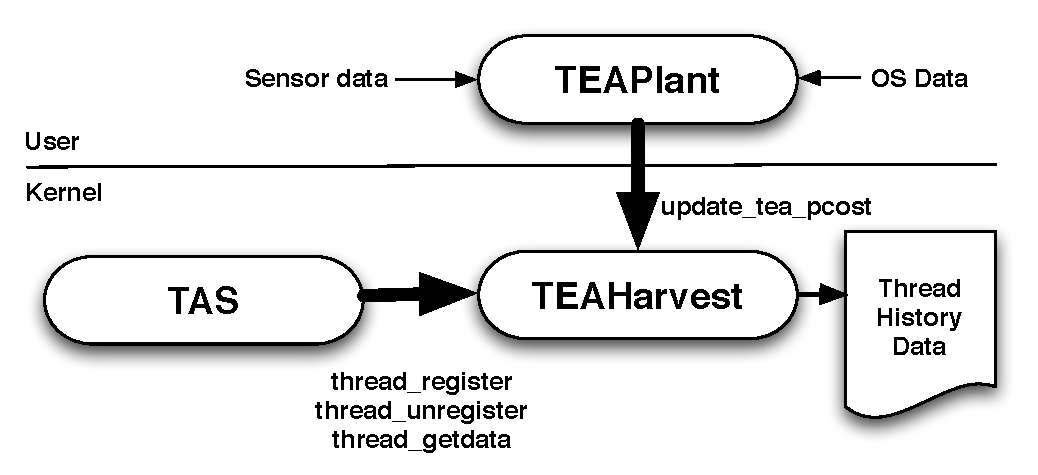
\includegraphics[scale=0.45]{tasdesign}
  \caption{TEAPlant and TEAHarvest data collection.}
  \label{fig:teaplant}
\end{figure}
\subsection{Thermal Predictors}
\label{sec:therm-pred-design} We enhance the existing operating system
to maintain information required by the thermal
estimator. Our design is based on the concept of Task Activity Vectors
(TAVs) introduced earlier \cite{Merkel2008a}.  A vector for each kernel
thread stores the required history needed to make sound prediction.
In general, one can trade additional space required by history maintenance
for the benefits gained from the thermal scheduling.

The high-level design of TAS is shown in \figurename~\ref{fig:teaplant}.
A user-level daemon process collects required information to compute
the time-series predictions for $\theta$ and $C_{theta}$. Temperature
readings are collected by this process from the digital temperature
sensor associated with a core.  Similarly, processor performance
counters are gathered by the same process, with both sets of metrics
used to generate estimates. Estimates are posted via a system call
interface to a device driver that collects the data for use by
the currently executing thread.  The scheduler queries this
driver via a kernel function call interface when making scheduling
decisions to determine the $\theta$ and $C_{\theta}$ estimates
associated with a thread.

\subsection{Thread Selection}
\label{sec:selection} The scheduler predicts a thread's impact on the
core temperature using the cost predictor for $C_{\theta}$
and accordingly adjusts the thread priority.  The TAS maintains three
queue structures per core: an idle queue, a current queue,
and the next queue. The core executes all work on the current
queue and then swaps its current queue and its next queue. For performance reasons,
our implementation follows the convention used by the existing
FreeBSD ULE scheduler, placing real-time and interrupt threads on the
current queue.

All other threads are scheduled in terms of an interactivity score.  In
the original ULE scheduler, the interactivity of a process was
determined by the formulas
\begin{equation}
  \label{eq:interactsleeprun} I = \dfrac{S}{\dfrac{SL}{RUN}}
\end{equation} and, for cases where thread's run time exceeds its sleep
time,
\begin{equation}
  \label{eq:interactrunsleep} I = \dfrac{S}{\dfrac{SL}{RUN}}+S
\end{equation} where $I$ is the interactivity score, $S$, the scaling
factor of the maximum interactivity score divided by two and $SL$ and
$RUN$ the respective cumulative sleep and run times for the thread.

For our TAS, this interactivity score is scaled by the predicted value
of $C_{\theta}$, normalized to a percentage value.  It was shown in
Zhou~\textit{et al.\ } \cite{Zhou2010b} that the greatest thermal
benefit occurs by selecting the thread to execute a scheduler should
favor the thread that moves the temperature as close as possible to a
DTM event without actually triggering that event.  The TAS achieves the
same effect by scaling the interactivity of the threads by the
normalized cost and, as result, gives less ``thermally costly'' threads
greater opportunity for access to the processor so as to moderate the
processor temperature.

\begin{figure}[t] \centering
  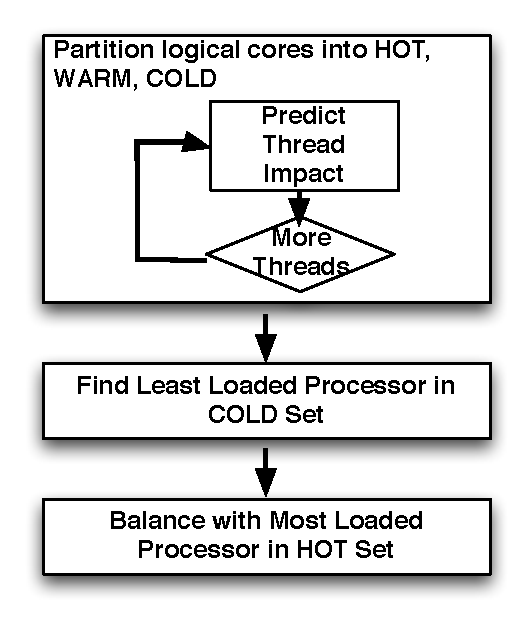
\includegraphics[scale=0.7]{tbalance.pdf}
  \caption{Design of thermal load balancing in TAS.}
  \label{fig:thermbal}
\end{figure}
\subsection{Load Balancing}
\label{sec:loadbalance} Load balancing distributes workload evenly
across the available logical CPUs; current implementations distribute to
maximize performance, we enhance the concept to distribute to minimize
thermal stress while seeking best performance. The TAS extends push
migration amongst processor groups by organizing the logical processors
in the system into three categories based upon the temperature at which
a DTM event occurs: Hot (90\% of DTM temperature), warm (between 75\%
and 90\% of DTM temperature), and cold (less than 75\% of the DTM
temperature).  In addition, we classify each logical CPU into ``clans''
depending whether a logical CPU is considered a ``fast processor'' or
``slow processor'' depending upon the current processor frequency of the
underlying hardware.  This two-level categorization allows us to manage
the distribution of work such that we can migrate work away from heat
sources while minimizing the impact on performance of threads.

For performance reasons, the thermal processor group topology is
maintained by the TEAHarvest thermal predictor driver.  The driver
allocates thermal efficiency and cost estimates to executing threads and
maintains the thermal processor group information. The TAS scheduler
queries the driver to determine whether a processor will move towards
the DTM temperature if a thread becomes ready to execute on the
appropriate run-queue.  In this way we predict whether a thread moves
the logical processor closer to a DTM event and adjust the processor
run-queue accordingly to prevent occurrence of the DTM event.

\begin{figure}[t] \centering
\begin{verbatim} 
BEGIN 
  Determine if the logical processor 
    is HOT, WARM, or COLD.  
  FOR each thread in the run queue 
     BEGIN 
        Project the resulting change 
           in temperature if 
           this thread executes.  
        Compute the projected logical CPU 
           speed over the elapsed 
           balance interval.  
      END 
  Determine the least loaded processor 
     in the ``COLD'' set.  
  Migrate the thread with 
     the ``worst'' impact on temperature 
     to the logical CPU in the COLD set most
     suitable from a speed standpoint.  
END
\end{verbatim}
  \caption{TAS balancing algorithm.}
  \label{fig:tascode}
\end{figure} 
On a periodic basis (every 500ms), the scheduler executes
the algorithm in \figurename~\ref{fig:tascode} in attempt to give
overtaxed resources additional time to thermally recover.  This
algorithm addresses thermal issues by moving the work away from
thermally stressed logical processors while attempting to maintain
system performance by selecting the logical processor with the least
load in the ``COLD'' set.

\section{Evaluation}
\label{sec:experiment} We evaluated our Thermal Aware Scheduler using
the FreeBSD operating system on commodity server hardware described in
Table~\ref{tab:hardware}. Our implementation modifies the existing the
push migration in FreeBSD's ULE scheduler~\cite{Roberson2003} to take
into account both thermal behavior and system performance per the
algorithms in Section~\ref{sec:sdesign}. PeC data is collected at the
user level using the standard tools provided for that purpose by FreeBSD
(the \texttt{coretemp} and \texttt{hwpmc} kernel extensions).  This
information is collected and collated by a FreeBSD kernel extension
which is queried by the operating system scheduler when making
scheduling decisions (\figurename~\ref{fig:teaplant})

The processor thermal model is calibrated by measuring the behavior of
the modified system at idle and under high load stress using common
utilities from the FreeBSD regression test suites and software
collections. Then, we characterize the CPU-related behavior of our
scheduler using integer and floating point benchmarks from the SPEC
CPU2006~\cite{Henning2006} benchmark suite. Finally, we use benchmarks
from the Princeton Application Repository for Shared-Memory Computers
(PARSEC) benchmark suite~\cite{Bienia2008} to consider the thread-level
and latency behavior of our scheduler.

\begin{table}[tbhp] \centering
  \caption{Server/Processor used in evaluation}
  \label{tab:hardware}
  \begin{tabular}{l l} 
\hline 
&\textbf{Dell Precision 490}\\ 
\hline
\hline 
CPU&Intel Xeon 5300 (Woodcrest)\\ 
CPU L2 cache&4MB\\ 
Memory&8GB,DDR2 667Mhz ECC\\
Internal disk&500GB\\ 
Network&1x1000Mbps\\ 
Video&NVIDA Quadro FX3400\\ 
\hline
  \end{tabular}
\end{table}
\subsection{Experiment Setup}
\label{sec:experiment-setup} Experiments were executed on the test
server specified in Table~\ref{tab:hardware}, with performance metrics
gathered during the course of execution. Power consumed is measured by a
WattsUP power meter \cite{WattsUp2006a}, connected between the AC Main
and the server under test.  The power meter measures the total and
average wattage, voltage, and amperage over the run of a workload.  The
internal memory of the power meter is cleared at the start of each run
and the measures collected during the runs are downloaded (after
execution completion) from meter's internal memory into a spreadsheet.

\subsection{Benchmark Selection Criteria}
\label{sec:experimental-setup-1} Components of the processor affect the
thermal envelope in different ways~\cite{Kumar2008}. We address this
issue by using three criteria for selecting benchmarks from the FreeBSD
stress testing, SPEC CPU 2006 and PARSEC benchmark suites
(Table~\ref{tab:benchmarks}): (1) sufficient coverage of the functional
units in the processor, (2) varying levels of CPU and memory intensity
to emulate real-life use of the processor, and (3) levels of reasonable
applicability to the problem space.

The benchmarks used in our evaluation address the first criteria in two
ways. The FreeBSD stress testing benchmarks operate by repeating a tight
set of integer and floating point instructions while doing multiple
reads and writes of large memory blocks.  This stresses the integer and
floating units in the processor while engaging in large amounts of cache
activity.  Further stress of the integer and floating points unit is
addressed by the balancing the selection of benchmarks from the SPEC
CPU2006 benchmark suite between integer and floating point benchmarks.

The second criteria is addressed by selecting benchmarks from the SPEC
CPU2006 and PARSEC suites that exhibit varying levels of CPU and memory
intensity.  This is demonstrated by (1) executed benchmarks singly to
focus upon each functional unit in the processor, and (2) executed in
combination across a mix of integer and floating point benchmarks
allocated across all logical processors in the system.  Finally, the
benchmarks were selected from the SPEC CPU2006 and PARSEC suites based
upon fit into the problem space.  Each benchmark represents an
application typical of the problems solved on high-performance
application servers.

\subsection{Calibration and Validation}
\label{sec:callibration} The thermal model in Section~\ref{sec:model}
was calibrated by comparing the behavior of each scheduler at idle
against behavior of the scheduler under heavy performance and thermal
stress. The system idle workload represents an idle operating system and
used as a frame of reference for comparing other workloads.  The
behavior of the system under high processor utilization and high memory
pressure was simulated using multiple instances of the FreeBSD
\texttt{cpuburn} stress testing package running in parallel, one per
core with symmetric multiple threads disabled.  The \texttt{cpuburn}
stress test package implements a single-threaded infinite loop with a
sequence of integer and floating-point operations to thermally stress a
processor.  These synthetic benchmarks was executed for 600 seconds with
PeCs in the model sampled at an interval of $t=5$ seconds.  Per the
procedure in \cite{Lewis2010}, these time-series observations were
consolidated using geometric means and chaotic attractor predictors were
built for the metrics in Section~\ref{sec:model}.

\begin{table}[tpbh]
  \caption{Benchmarks used for evaluation}
  \label{tab:benchmarks} 
\centering
\begin{tabular}{c c p{5cm}} 
\hline 
\hline
\multicolumn{3}{l}{\textbf{Integer Benchmarks}}\\ 
\hline 
% BEGIN RECEIVE ORGTBL intbench 
hmmer &  & Search gene sequence \\
mcf &  & Combinatorial optimization \\
% END RECEIVE ORGTBL intbench 
\hline 
\hline
\multicolumn{3}{l}{\textbf{Floating Benchmarks}}\\ 
\hline 
%BEGIN RECEIVE ORGTBL fpbench
milc &  & Quantum Chromodynamics \\
gromacs &  & Biochemistry/MolecularDynamics \\
libquantum &  & Physics/General Relativity \\
namd &  & Fluid Dynamics \\
%END RECEIVE ORGTBL fpbench
\hline
\end{tabular} % system benchmark table
\begin{comment} % integer benchmark table
\begin{comment} 
#+ORGTBL: SEND intbench orgtbl-to-latex :splice t :skip 0 
| hmmer |   | Search gene sequence       |
| mcf   |   | Combinatorial optimization |
\end{comment} 
% Floating point benchmark table
\begin{comment} 
#+ORGTBL: SEND fpbench orgtbl-to-latex :splice t :skip 
| milc       |   | Quantum Chromodynamics         |
| gromacs    |   | Biochemistry/MolecularDynamics |
| libquantum |   | Physics/General Relativity     |
| namd       |   | Fluid Dynamics                 |
\end{comment}
\end{table}
\subsection{CPU-Bound Behavior}
\label{sec:microarch} It has been shown in prior work
\cite{Choi2007,Cher2011} that significant core-to-core and functional
unit-to-functional unit thermal variation occurs on modern processors.
Benchmarks from the SPEC CPU2006 suite \cite{Spec2006}, (as listed in
Table~\eqref{tab:benchmarks}), were used to compare the thermal behavior
of CPU-bound workloads executed on the TAS scheduler vs. same workload
for the ULE scheduler.

\begin{figure}[!tbhp] \centering
  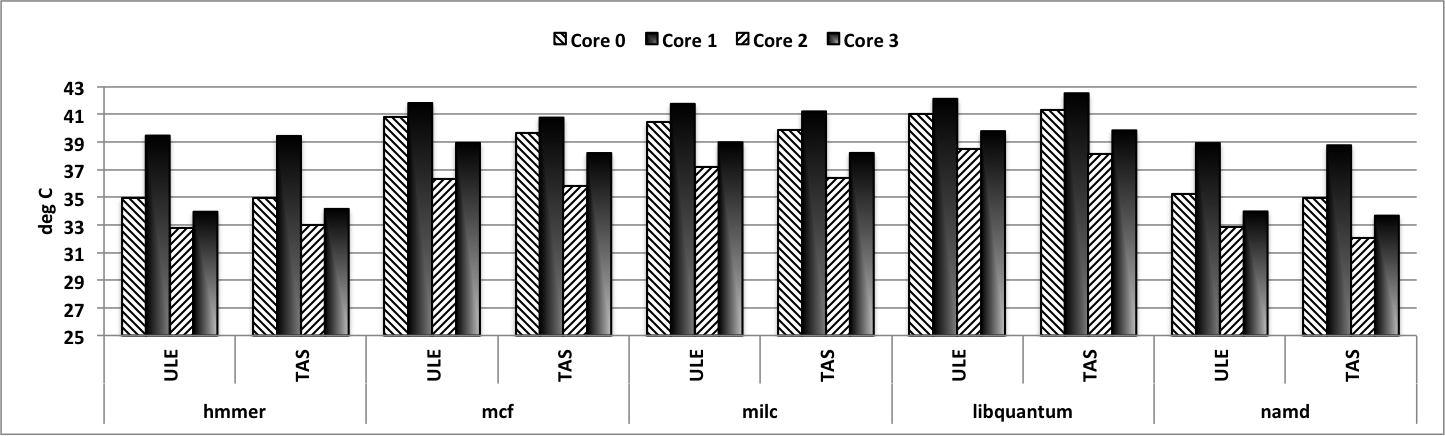
\includegraphics[width=1.0\linewidth,height=2in]{graphics/speccputemp}
  \caption{Average core die temperature under selected SPEC CPU20006
benchmarks for ULE and TAS schedulers.}
  \label{fig:ubenchmarks}
\end{figure} 
In \figurename~\ref{fig:ubenchmarks}, we see the average
core die temperature for each processor in our test system for each of
the benchmarks in Table~\ref{tab:benchmarks}.  We see very little
temperature variation between the two schedulers in this case as these
benchmarks are CPU-bound which means that threads for these processes
tend to congregate on the same core due to cache affinity.  Thus, the
lack of temperature variation as the TAS adjusts its thread selection to
minimize the impact in performance for workloads of this type.

\begin{table}[bp]
  \caption{Cross-functional unit benchmark combinations}
  \label{tab:crossbench}b \centering
  \begin{tabular}{clllll} \hline Workload & & Thread 0 & Thread 1 &
Thread 2 & Thread 3 \\ \hline \hline A & & namd & namd & hmmer & mcf \\
B & & milc & milc & namd & hmmer \\ C & & milc & mcf & mcf & hmmer \\
\hline
  \end{tabular}
\end{table}
\subsubsection{Cross-Functional Unit Evaluation}
\label{sec:cross-funct-unit} In this section, we consider the effect of
mixed workloads multi-threading across multiple logical processors.  We
construct mixed workloads from combinations of the the SPEC CPU2006
benchmarks that span a range of cases including high-IPC/low-IPC,
hot/cold thermal profiles (per \cite{Kursun2008}), and
integer/floating-point combinations (Table~\ref{tab:crossbench}). A
single copy of each benchmark was executed in parallel with the
operating system making the decision as to where to execute the
workload.  It was observed that as the workload progressed, the executed
threads again tended to pin themselves to a particular core depending
upon thread use of cache and memory.

\begin{table}[!bp] 
\centering
  \caption{Cross-functional unit execution}
  \label{tab:mixwkload}
  \begin{tabular}{cllllll} 
% BEGIN RECEIVE ORGTBL mixwkload \hline
\hline
Workload & Core 0 & Core 1 & Core2 & Core 3 & Perf. \\
 &  &  &  &  & Impact \\
\hline
\hline
A & 6.0\% & 2.1\% & 3.9\% & 4.5\% & 2.1\% \\
B & 2.2\% & 1.7\% & 4.8\% & 2.5\% & 2.9\% \\
C & 6.9\% & 7.1\% & 7.1\% & 6.5\% & 2.5\% \\
\hline
% END RECEIVE ORGTBL mixwkload
  \end{tabular}
\begin{comment} 
#+ORGTBL: SEND mixwkload orgtbl-to-latex :splice t :skip 0 
|----------+--------+--------+-------+--------+--------|
| Workload | Core 0 | Core 1 | Core2 | Core 3 | Perf.  |
|          |        |        |       |        | Impact |
|----------+--------+--------+-------+--------+--------|
|----------+--------+--------+-------+--------+--------|
| A        | 6.0\%  | 2.1\%  | 3.9\% | 4.5\%  | 2.1\%  |
| B        | 2.2\%  | 1.7\%  | 4.8\% | 2.5\%  | 2.9\%  |
| C        | 6.9\%  | 7.1\%  | 7.1\% | 6.5\%  | 2.5\%  |
|----------+--------+--------+-------+--------+--------|
\end{comment}
\end{table} In this experiment, we see temperature improvements between
1.7\% and 7.1\% (as shown in Table~\ref{tab:mixwkload}) with a
performance impact of between 2.1\% and 2.9\%.  This compares favorably
with techniques from prior work such as Core Hopping~\cite{Choi2007},
Variation-Aware~\cite{Kursun2008}, and Predict-and-Act~\cite{Ayoub2009},
with comparable reductions in average core die temperatures and
performance impact for similar workloads and processors.

\begin{figure}[!tbp] 
\centering
  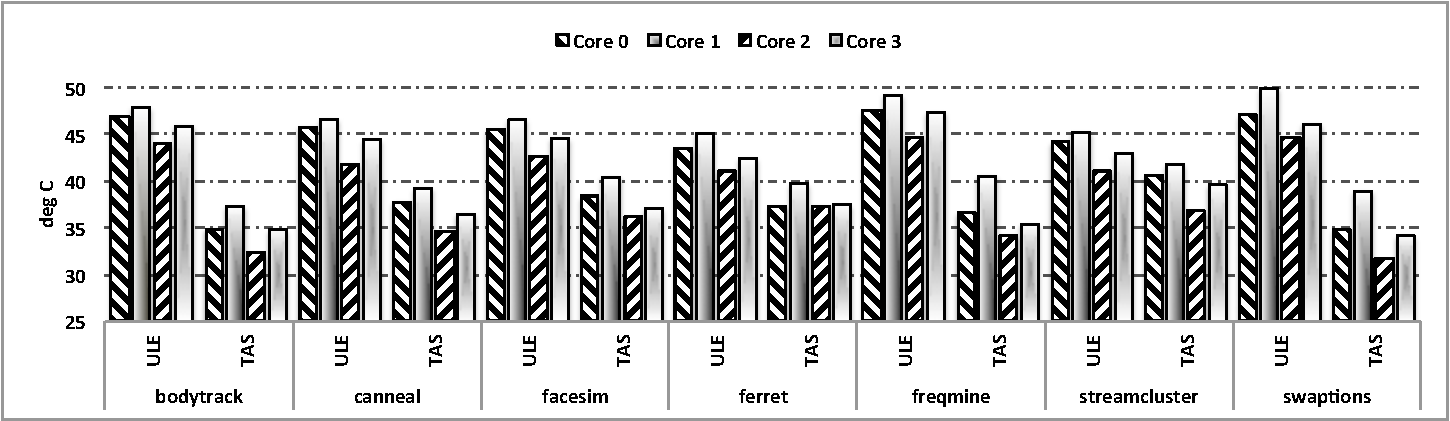
\includegraphics[width=1.0\linewidth,height=2in]{graphics/parsectemp}
  \caption{Comparison of PARSEC benchmark average core die temperatures
under ULE and TAS schedulers.}
  \label{fig:pbenchmarkt}
\end{figure}
\begin{table}[!b] 
\centering
  \caption{PARSEC benchmarks used in evaluation}
 \label{tab:parsecbench}
  \begin{tabular}[bthp]{c c p{5cm}} 
   \hline \hline 
     % BEGIN RECEIVE ORGTBL parsecbench 
blackscholes &  & Black-Scholes PDE solver for options analysis \\
bodytrack &  & Computer vision image tracking application \\
canneal &  & Simulated annealing chip routing cost computation \\
facesim &  & Physical simulation of facial behavior \\
ferret &  & Content-based similarity search \\
fluidanimate &  & Animation of fluid dynamics \\
freqmine &  & Simulate FP-growth method for Frequent Itemset Mining \\
streamcluster &  & Online clustering algorithm for data mining \\
swaptions &  & Simulated pricing of portfolio options \\
     % END RECEIVE ORGTBL parsecbench 
\hline
\end{tabular}
\begin{comment} 
#+ORGTBL: SEND parsecbench orgtbl-to-latex :splice t :skip 0 
| blackscholes  |   | Black-Scholes PDE solver for options analysis         |
| bodytrack     |   | Computer vision image tracking application            |
| canneal       |   | Simulated annealing chip routing cost computation     |
| facesim       |   | Physical simulation of facial behavior                |
| ferret        |   | Content-based similarity search                       |
| fluidanimate  |   | Animation of fluid dynamics                           |
| freqmine      |   | Simulate FP-growth method for Frequent Itemset Mining |
| streamcluster |   | Online clustering algorithm for data mining           |
| swaptions     |   | Simulated pricing of portfolio options                |
\end{comment}
\end{table}
\subsection{Multi-threaded behavior}
\label{sec:mult-behav} We evaluate behavior of our scheduling algorithms
when executing highly parallel workloads using selected benchmarks from
the PARSEC~\cite{Bienia2008} suite. Benchmarks in this suite use
different combinations of parallel workloads selected from the fields of
computer vision, computational finance, enterprise servers, and
animation physics as described in Table~\ref{tab:parsecbench}.  The
benchmarks were compiled with the POSIX \texttt{pthreads} library and
executed using the PARSEC \texttt{native} input sets.

\begin{figure}[!tbp]
  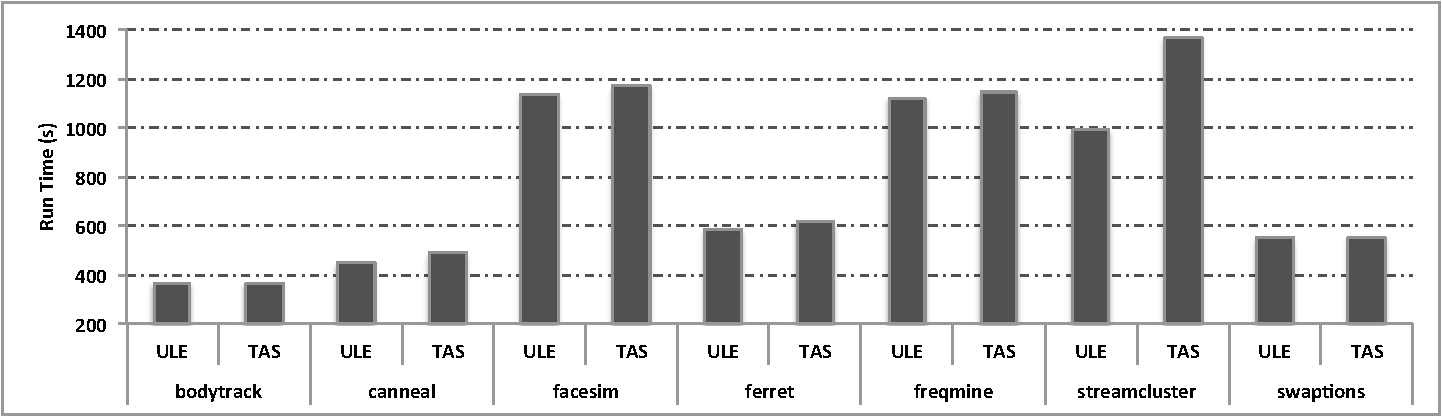
\includegraphics[width=1.0\linewidth,height=2in]{graphics/parsecperformance}
  \caption{Comparison of PARSEC benchmark performance under ULE and TAS
schedulers.}
  \label{fig:pbenchmarkp}
\end{figure} 
Three metrics were used to compare the behavior oF the ported PARSEC
benchmarks for the original ULE scheduler and our TAS: (a) the average
core die temperature (\figurename~\ref{fig:pbenchmarkt}), (b) benchmark
performance (\figurename~\ref{fig:pbenchmarkp}), and (c) average system
power (\figurename~\ref{fig:pbenchmark}).  We see improved performance
from benchmarks such as \texttt{bodytrack} and \texttt{swaptions} that utilize
smaller working sets and consequently have less need for bigger cache
capacity~\cite{Bienia2011} with TAS showing an improvement of
10-12$^{\circ}$C.\ with a minimal impact on performance.  Benchmarks
with streaming behavior such as\texttt{facesim}, \texttt{freqmine}, or
\texttt{streamcluseter} with much larger working sets demonstrate less
improvement with TAS, with average core die temperature differences 3-6$^{\circ}$C.\ less
than ULE.

\begin{figure}[!tbp]
  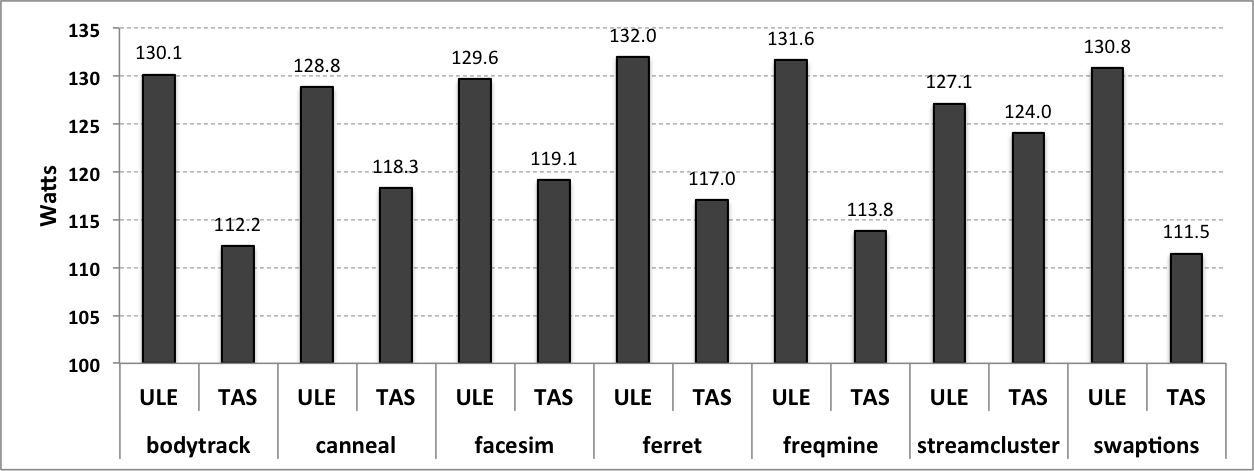
\includegraphics[width=1.0\linewidth,height=2in]{ParsecPowerConsumption.png}
  \caption{Comparison of PARSEC benchmark average power consumption under ULE and TAS schedulers.}
  \label{fig:pbenchmark}
\end{figure}
In \figurename~\ref{fig:tasvsedp}, we contrast the optimization strategy
used by TAS versus other possible optimizations schemes for managing the
trade-off between performance and energy.  In this figure, we compare
TAS performance results from executing the PARSEC
\texttt{facesim} benchmark as compared to schemes that minimize delay
under peak power constraints (DPC) and minimize energy under peak power and
delay constraints (EPDC). DPC minimizes the delay of an execution
interval so that the maximum power within an execution interval never
exceeds a limit while EPDC schemes seek to minimize energy while
operating a system within a power budget with a limit on the workload
performance impact. In this case, the optimizations used by TAS
outperforms both DPC and EPDC for the \texttt{facesim} 
benchmark by 4\% to 6\%  as reported in prior work~\cite{Cochran2011}. 

\begin{figure}[!tbhp]
  \centering
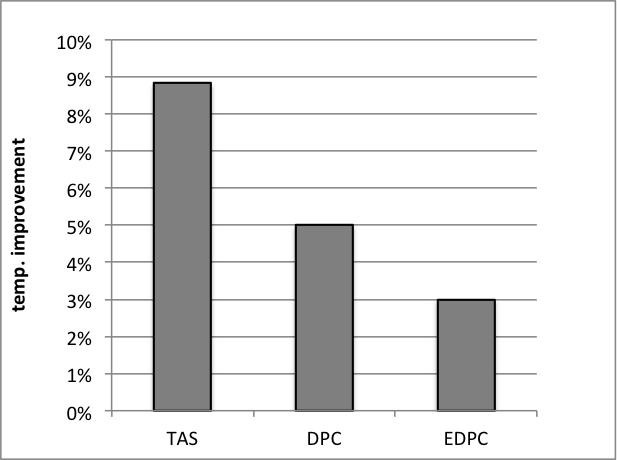
\includegraphics[scale=0.6]{graphics/tasvsedpc}
  \caption{Average percentage reduction in core die temperature for the
    \texttt{facesim} benchmark under various optimization strategies.}
  \label{fig:tasvsedp}
\end{figure}
\section{Conclusion}
\label{sec:conclusion}
Dense servers pose power and thermal challenges that pose problems for
processor that crude methods such as DVFS and DTM do not address in an
effective and efficient manner.   As result, system performance can be
compromised when such servers are highly utilized.   In this work, we
have presented pro-active scheduling techniques that utilize thermal
Chaotic Attractor Predictors that take into account key thermal
indicators and system performance metrics to guide thread selection  and
load balancing.  We have developed an effective thread scheduler for
multicore systems that manages system energy consumption withing a given
power and thread envelope. It was found through experimental validation
that these techniques are capable of reducing the average on-die core
temperatures of a typical server processor between 3 to 6$^{\circ}$C.\ for
benchmarks that exhibit streaming behavior and 10-12$^{\circ}$C.\ for
other benchmarks with minimal impact on performance.

\label{sec:references}
\bibliographystyle{ULieeetran}
\bibliography{../overall.bib}
\end{document}
% The following comment block is used by the different flavors of EMACS and
% the AUCTEX package to manage multiple documents.  In order for AUCTEX
% to understand you're working with multiple files, you should define
% the TeX-master variable as a file local variable that identifies your
% master document.
%
% Please do not remove.
%%% Local Variables: 
%%% mode: latex
%%% TeX-master: "scheduler.tex"
%%% TeX-PDF-mode: t
%%% TeX-source-correlate-mode: t
%%% End: 
